\chapter{A meta-analysis of FUS splicing comparing knockouts with patient-like $\Delta$NLS mutations}
\label{chapter:fus_meta}

\section{Background}

FUS


\begin{figure}[h!]
	\centering
	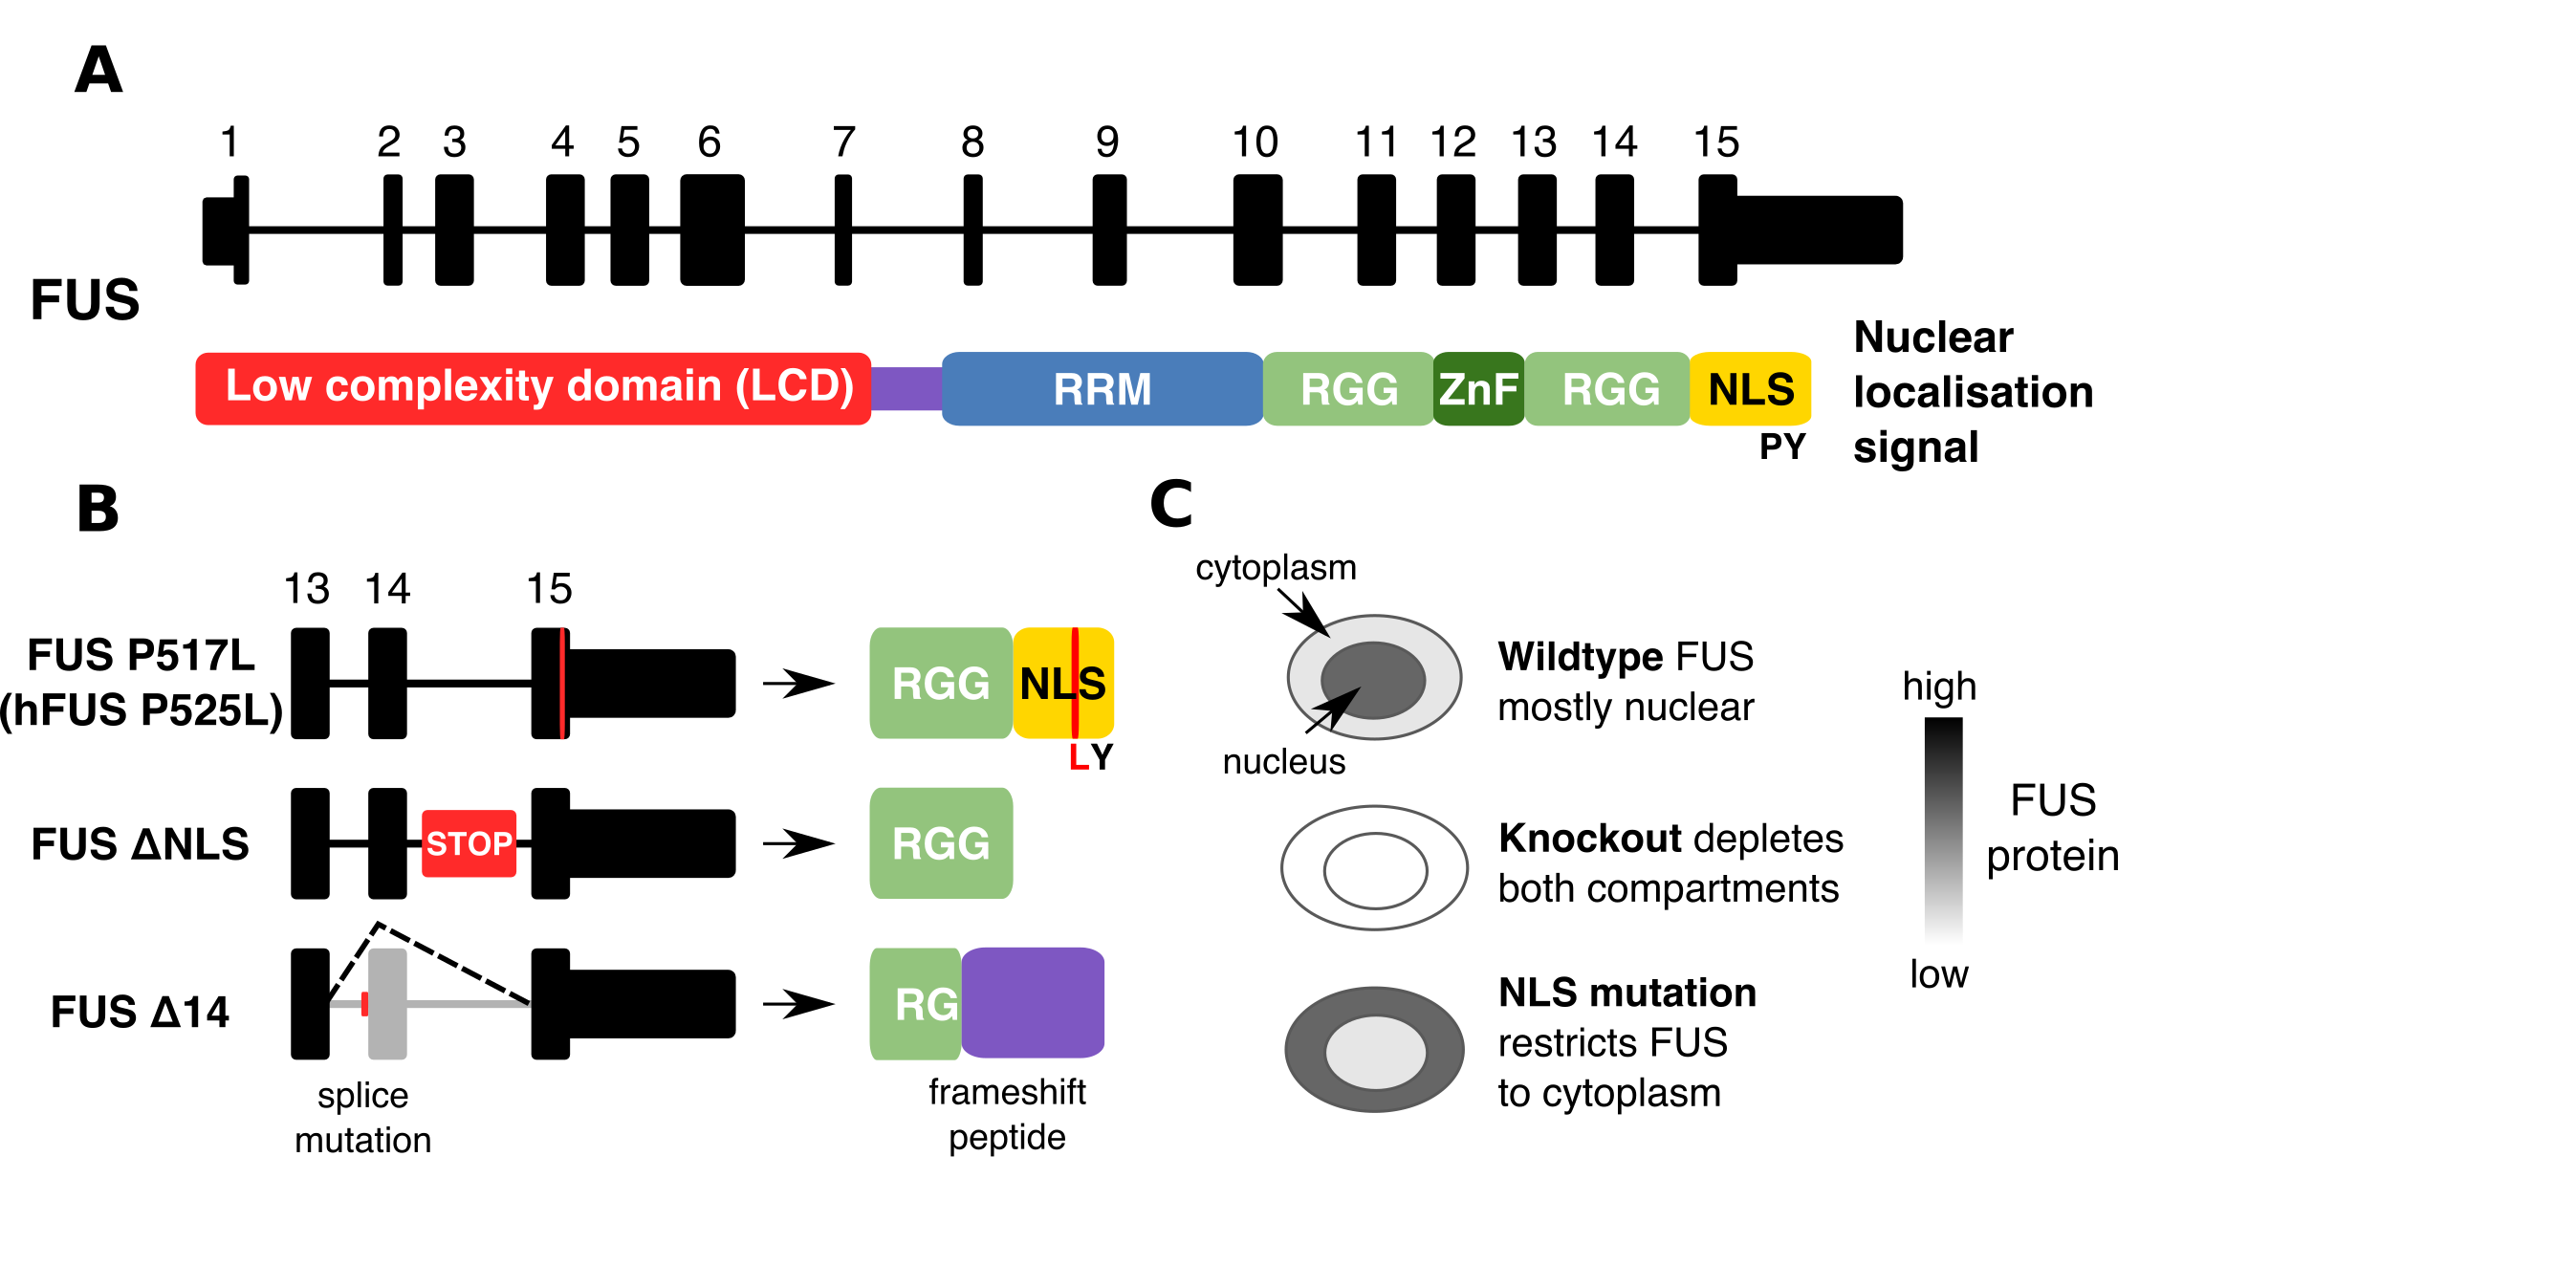
\includegraphics[width=\textwidth]{Figures/06_fus_meta/FUS_structure_mutations.png}
	\caption{\textbf{The structure of the FUS protein and known ALS mutations}}
	A: FUS is comprised of a low complexity domain (LCD), an RNA recognition motif (RRM) domain, two Arginine-Glycine-Glycine (RGG) domains, a zinc finger domain (Znf), a nuclear export signal (NES) and a nuclear localisation signal (NLS). The P525L mutation is highlighted in bold type. Schem	atic adapted from \citep{Shang2016}.
	B: In wildtype (+/+) cells FUS protein is predominantly nuclear but can shuttle to the cytoplasm. When FUS is knocked out or down it will be reduced in both compartments but if the nuclear localisation signal (NLS) is mutated or deleted then FUS will accumulate in the cytoplasm although some will enter the nucleus.
	\label{fig:fus_structure}
\end{figure}




\section{Contributions}
RNA sequencing libraries prepared by Dr Nicol Birsa
Mice handled by Dr Cristian Bodo
RNA extracted for PCR by Dr Nicol Birsa and Matthew Bentham
RT-PCRs performed by David Robaldo and Dr Carmelo Milioto

All bioinformatic analysis and interpretation was performed by myself. 

\section{Background}

% importance of NLS to FUS

Delta 14 - very aggressive
P525L - Patients with the P525L mutation die at a much younger age than patients with any other FUS mutation \citep{Shang2016}.


\section{Methods}

\subsection{Data processing}
Usual pipeline. Aligned with STAR, reads counting with HTSeq-count. 

\subsection{Differential Expression}
DESeq2 \citep{Love2014}
Model all data together with a dataset covariate to maximise power.
Extract condition specific fold changes (Wald test). False Discovery Rate threshold of 5\% applied. Shrunken fold change values reported. Gene expression values are plotted as raw counts multiplied by each samples’ size factor generated by DESeq2.

\subsection{Differential Splicing}
SGSeq (Goldstein) \citep{Goldstein2016}] to discover and classify splicing variants. Differential splicing was tested using DEXSeq \cite{Anders2012}.
Group data into conditions and model fold change per comparison. SGSeq looks for all potential splicing variants in each sample and then counts the reads supporting each the inclusion or exclusion of that splicing variant. 
Percentage Spliced In (PSI) values (Katz) \citep{Katz2010-ir} for each splicing variant were calculated by taking the read counts supporting the inclusion event and dividing by the total reads in that event. 

For individual splicing events, PSI values were compared between each condition using a one-way ANOVA with post-hoc Tukey test.

\subsection{Gene Ontology}
GProfileR package \citep{Reimand2016}. GO categories were hand-curated and restricted to at least 5 genes per set. P-values reported after Bonferroni correction. 

\subsection{Polyadenylation and iCLIP}
PolyAsite mm10 v1.0 \citep{Gruber2016} . Each site must be supported by at least 2 datasets.
iCLIP data from Rogelj via iCOUNT .

\subsection{Conservation}
Per nucleotide PhyloP conservation scores (Pollard) \citep{Pollard2010-fj} comparing mouse (mm10) with 60 ??? animals was downloaded from UCSC. For each splicing variant the entire length of the encompassing intron was taken and the median PhyloP score calculated.

\subsection{RT-PCR}
Primers were designed using Primer3 \citep{Koressaar2007} and in silico PCR (UCSC). 
For both human and mouse FUS, the forward primer was designed for exon 6 and the reverse primer designed to span the spliced exon 8/9 junction to preferentially amplify spliced FUS RNA. 
An additional third primer was designed to amplify a section of either intron 6 or intron 7.

Cells were obtained from mouse brains and/or cultured mouse embryonic fibroblasts resuspended in trizol. 
RNA was extracted using miRNeasy Mini Kit (Qiagen) following the manufacturer’s instructions % what kit did Nicol use?
cDNA was obtained from extracted RNA using SuperScript IV Reverse Transcriptase kit (Invitrogen). 
Briefly, a mix was made of RNA template (500ng for mouse brain; 100ng for cultured cells (cycloheximide treatment), 10 mM dNTP, 50 mM oligo d(T)20, 50 mM random hexamer followed by 5 min of incubation at 65$\degree$C and 1 min in ice. Mix was then complemented with 5X SuperScript IV Reverse Transcriptase buffer, 100 nM DTT, RNase OUT and SuperScript IV Reverse Transcriptase buffer followed by incubation at 23$\degree$C, 55$\degree$C and 80$\degree$C, 10 min each. 

RT-PCR was carried out using 10X AccuPrime Taq DNA polymerase mastermix system (Invitrogen). 
Each PCR reaction mix contained 5 ng of gDNA, 10 mM of forward and reverse primers. cDNA was amplified with the following conditions:
Intron 6 retention: One cycle of 5 min at 95$\degree$C, followed by 30 cycles of 30 sec at 95$\degree$C, 30 sec at 56$\degree$C, and 30 sec at 68$\degree$C, and finishing with 5 min incubation at 68$\degree$C.
Intron 7 retention: One cycle of 5 min at 95$\degree$C, followed by 30 cycles of 30 sec at 95$\degree$C, 30 sec at 61$\degree$C, and 30 sec at 68$\degree$C, and finishing with 5 min incubation at 68$\degree$C.
Srsf7 NMD positive control: One cycle of 5 min at 95 $\degree$C, followed by 35 cycles of 30 sec at 95 $\degree$C, 30 sec at 58 $\degree$C, and 15 sec at 68 $\degree$C, and finishing with 5 min incubation at 68 $\degree$C.
Amplified products were finally obtained using Agilent 4200 TapeStation System following the manufacturer’s instructions. Results were analysed on TapeStation analysis software.
Intron retention events are plotted  as the percentage of integrated area of the retained band.

FUCK MEC

\begin{table}[h!]
	%\begin{centerline}
	\centering
	\begin{tabular}{rcl}
		\textbf{Target} & \textbf{Direction} & \textbf{Sequence}\\
		\hline \\[-0.3cm]
		mFUS exon 6  & F &  GTTATGGCAATCAGGACCAGAG\\
		mFUS intron 6 & R & TTGGCTCCCAAGTTCTCACA\\
		mFUS intron 7 & F &  GGAGAAACTGGATGGATGCAC\\
		mFUS exon 8/9 & R &  CCTGTTCAGAATCATGACGAGA\\[0.2cm]
		hFUS exon 6 & F & TCCTCCATGAGTAGTGGTGGT \\
		hFUS intron 6 & R & GTTCAGGCTCCCAAGTTCTC\\
		hFUS intron 7 & F & TTCTCTCGGGTGAGAGAACC\\
		hFUS exon 8/9 & R & GTCTGAATTATCCTGTTCGGAGTC\\[0.2cm]
		mSRSF7 & F &  CGACGAAGAAGAAGCAGGTTTC\\
		mSRSF7& R & TCTGGCCTCTTATGCTGATCAC\\
	\end{tabular}
	%\end{centerline}
	\caption{List of primers used in RT-PCR. mFUS: mouse \textit{FUS}; hFUS: human \textit{FUS}}
	\label{tab:fus_primers}
\end{table}




\subsection{Cycloheximide treatment}
Mouse embryonic fibroblasts were treated with 100ug/ml cycloheximide for 6 hours before RNA was extracted with Trizol (Thermo Fisher) and RT-PCR performed as before. 


\clearpage



\section{Results}

\subsection{ Comparing three RNA-seq dataset of FUS knockout and FUS mutation}

% Discuss 3 datasets, pros and cons of each
% differences in sequencing, prediction
Three dataset generated
%Dupuis
The lab of Luc Dupuis from INSERM, Strasbourg generated RNA-seq data from mouse embryonic brain (day E18.5). Their knockout construct uses a gene trap (citation?) in intron 1 generated by themselves as they argue this creates a more effective knockout than previous gene traps.  
Their NLS mutation introduces a stop codon after exon 14, terminating transcription upstream of the NLS sequence. 
All mice are homozygous for their transgenes. 
The two conditions have their own separate wildtype littermate controls. 
The depth and read length of the RNA-seq libraries is shorter than the other two datasets but this is compensated for by being polyA+ enriched, which will mean a greater proportion of sequencing reads aligning to coding exons.  
This will be useful for assessing differential expression but I predict the dataset will not be particularly useful for differential splicing.
The Dupuis dataset was published as \citep{Scekic-zahirovic2016}.

% Bozzoni
The lab of Irene Bozzoni at the University of Rome generated RNA-seq data from purified motor neurons cultured from mouse induced pluripotent stem cells. Their knockout uses a gene trap in exon 12 first used in \citep{Hicks2000}. 
This is the knockdown claimed to be weak by the Dupuis group.
Again all mice are homozygous for their transgenes.
Their NLS mutation is a point mutation affecting the penultimate amino acid of the NLS which in humans is the very aggressive ALS mutation P525L, which translates in mice to P517L.  
The two conditions share a single set of controls, which are motoneurons derived from wildtype stem cells.
The read depth and length is moderately high but the sample number is on the lower side (n=3 for each condition).
The Bozzoni dataset was published as \citep{Capauto2018}.

% Fratta
The third dataset was generated in-house by the lab of Pietro Fratta using mouse embryonic spinal cords (embryonic day E18.5). The knockout construct is the same as the Dupuis dataset so should be a robust knockout of FUS. 
The NLS mutation is the $\Delta$14 mutation discussed in \autoref{chapter:fus_mouse}, where a splice site mutation prevents the inclusion of exon 14, causing a downstream frameshift and ablation of the entire NLS. 
The wildtype littermate controls are separate for each condition. 
The RNA-seq data produced is of the highest quality of the three, with 150bp reads and high depth. 
This will be useful in quantifying differential splicing, although as it is total RNA rather than polyA+ enriched there will be a lot of pre-mRNA present.
The Fratta dataset is unpublished.





\begin{longtable}[]{@{}llllll@{}}
	\begin{minipage}[t]{0.14\columnwidth}\raggedright\strut
		{\textbf{Dataset}}\strut
	\end{minipage} & \begin{minipage}[t]{0.14\columnwidth}\raggedright\strut
		{\textbf{Tissue}}\strut
	\end{minipage} & \begin{minipage}[t]{0.12\columnwidth}\raggedright\strut
		{\textbf{Controls}}\strut
	\end{minipage} & \begin{minipage}[t]{0.10\columnwidth}\raggedright\strut
		{\textbf{Age}}\strut
	\end{minipage} & \begin{minipage}[t]{0.14\columnwidth}\raggedright\strut
		{\textbf{Knockout (KO)}}\strut
	\end{minipage} & \begin{minipage}[t]{0.14\columnwidth}\raggedright\strut
		{\textbf{Mutation (MUT)}}\strut
	\end{minipage}\tabularnewline\toprule \\[-0.3cm] 
	\begin{minipage}[t]{0.16\columnwidth}\raggedright\strut
		{\textbf{Dupuis}}
		{\footnotesize\citep{Scekic-zahirovic2016}}\strut
	\end{minipage} & \begin{minipage}[t]{0.14\columnwidth}\raggedright\strut
		{Whole brain}\strut
	\end{minipage} & \begin{minipage}[t]{0.12\columnwidth}\raggedright\strut
		{Separate}\strut
	\end{minipage} & \begin{minipage}[t]{0.10\columnwidth}\raggedright\strut
		{E18.5}\strut
	\end{minipage} & \begin{minipage}[t]{0.16\columnwidth}\raggedright\strut
		{Gene trap in intron 1}\strut
	\end{minipage} & \begin{minipage}[t]{0.16\columnwidth}\raggedright\strut
		{Stop codon after exon 14 ($\Delta$NLS)}\strut
	\end{minipage}\tabularnewline \\
	\begin{minipage}[t]{0.16\columnwidth}\raggedright\strut
		{\textbf{Bozzoni}}
		{\footnotesize\citep{Capauto2018}}\strut
	\end{minipage} & \begin{minipage}[t]{0.14\columnwidth}\raggedright\strut
		{Motor neurons}
		{cultured from iPSCs}\strut
	\end{minipage} & \begin{minipage}[t]{0.12\columnwidth}\raggedright\strut
		{Shared}\strut
	\end{minipage} & \begin{minipage}[t]{0.10\columnwidth}\raggedright\strut
		{-}\strut
	\end{minipage} & \begin{minipage}[t]{0.16\columnwidth}\raggedright\strut
		{Gene trap in exon 12}
		
		{ \footnotesize\citep{Hicks2000} }\strut
	\end{minipage} & \begin{minipage}[t]{0.16\columnwidth}\raggedright\strut
		{P517L knock-in,}
		{corresponding to human P525L}
		{\footnotesize\citep{Conte2012}}\strut
	\end{minipage}\tabularnewline \\
	\begin{minipage}[t]{0.16\columnwidth}\raggedright\strut
		{\textbf{Fratta}}\strut
	\end{minipage} & \begin{minipage}[t]{0.14\columnwidth}\raggedright\strut
		{Spinal cord}\strut
	\end{minipage} & \begin{minipage}[t]{0.12\columnwidth}\raggedright\strut
		{Separate}\strut
	\end{minipage} & \begin{minipage}[t]{0.10\columnwidth}\raggedright\strut
		{E18.5}\strut
	\end{minipage} & \begin{minipage}[t]{0.16\columnwidth}\raggedright\strut
		{Gene trap in intron 1}\strut
	\end{minipage} & \begin{minipage}[t]{0.16\columnwidth}\raggedright\strut
		{$\Delta$ exon 14 }
		{\footnotesize\citep{Devoy2017}}  \strut
	\end{minipage}\tabularnewline
	\caption{The three FUS mouse datasets}
	\label{tab:fus_datasets}
\end{longtable}

% SEQUENCING STATS

\begin{longtable}[]{@{}llllll@{}}
	\begin{minipage}[t]{0.14\columnwidth}\raggedright\strut
		{\textbf{Dataset}}\strut
	\end{minipage} & \begin{minipage}[t]{0.14\columnwidth}\raggedright\strut
		{\textbf{Replicates per condition}}\strut
	\end{minipage} & \begin{minipage}[t]{0.14\columnwidth}\raggedright\strut
		{\textbf{Library type}}\strut
	\end{minipage} & \begin{minipage}[t]{0.14\columnwidth}\raggedright\strut
		{\textbf{Mapped reads (millions)}}\strut
	\end{minipage} & \begin{minipage}[t]{0.14\columnwidth}\raggedright\strut
		{\textbf{Read type}}\strut
	\end{minipage} & \begin{minipage}[t]{0.14\columnwidth}\raggedright\strut
		{\textbf{SRA accession}}\strut
	\end{minipage}\tabularnewline\toprule \\[-0.3cm]
	\begin{minipage}[t]{0.14\columnwidth}\raggedright\strut
		{\textbf{Dupuis}}\strut
	\end{minipage} & \begin{minipage}[t]{0.14\columnwidth}\raggedright\strut
		{4-5}\strut
	\end{minipage} & \begin{minipage}[t]{0.14\columnwidth}\raggedright\strut
		{mRNA}\strut
	\end{minipage} & \begin{minipage}[t]{0.14\columnwidth}\raggedright\strut
		{15-25}\strut
	\end{minipage} & \begin{minipage}[t]{0.14\columnwidth}\raggedright\strut
		{1 x 50bp}\strut
	\end{minipage} & \begin{minipage}[t]{0.14\columnwidth}\raggedright\strut
		{SRP070906 }\strut
	\end{minipage}\tabularnewline \\
	\begin{minipage}[t]{0.14\columnwidth}\raggedright\strut
		{\textbf{Bozzoni} }\strut
	\end{minipage} & \begin{minipage}[t]{0.14\columnwidth}\raggedright\strut
		{3}\strut
	\end{minipage} & \begin{minipage}[t]{0.14\columnwidth}\raggedright\strut
		{Total RNA}\strut
	\end{minipage} & \begin{minipage}[t]{0.14\columnwidth}\raggedright\strut
		{34-52}\strut
	\end{minipage} & \begin{minipage}[t]{0.14\columnwidth}\raggedright\strut
		{2 x 100bp}\strut
	\end{minipage} & \begin{minipage}[t]{0.14\columnwidth}\raggedright\strut
		{SRP111475}\strut
	\end{minipage}\tabularnewline \\
	\begin{minipage}[t]{0.14\columnwidth}\raggedright\strut
		{\textbf{Fratta} }\strut
	\end{minipage} & \begin{minipage}[t]{0.14\columnwidth}\raggedright\strut
		{4}\strut
	\end{minipage} & \begin{minipage}[t]{0.14\columnwidth}\raggedright\strut
		{Total RNA}\strut
	\end{minipage} & \begin{minipage}[t]{0.14\columnwidth}\raggedright\strut
		{52-65}\strut
	\end{minipage} & \begin{minipage}[t]{0.14\columnwidth}\raggedright\strut
		{2 x 150bp}\strut
	\end{minipage} & \begin{minipage}[t]{0.14\columnwidth}\raggedright\strut
		{-}\strut
	\end{minipage}\tabularnewline
	\caption{RNA-seq statistics of the three datasets}
	\label{tab:fus_sequencing}
\end{longtable}




\subsection{Modelling differential expression jointly boosts power and demonstrates significant overlap between KO and MUT}

% Explain individual analyses

Differential expression compares the abundances of each gene's RNA between two conditions. As most RNA-sequencing datasets comprise small numbers of samples, the number of genes found to be significantly changed between conditions highly depends on the degree of difference between conditions, the number of samples per condition, and the read depth covering each gene. The more sequencing reads that cover a gene, the more precise the measure of the true variance can be.
Most software packages attempt to get round these hurdles by borrowing information across all genes to shrink the variance between samples of the same condition. 
When I analyse each dataset individually, comparing KO and MUT to their respective controls in each dataset, the Dupuis dataset has the largest number of differentially expressed genes in both conditions. 
This is probably due to a larger sample size and the fact that their data is polyA+ enriched, which will potentially reduce the between-sample variation allowing for more precise measures of between-condition differences. 
It is also possible that however they prepared the tissues and extracted the RNA resulted in less variability between samples.
Despite the differences in numbers, in all three datasets the KO condition produces more differentially expressed genes than MUT, suggesting a stronger effect of knocking out FUS than mutating the NLS.


% Combining datasets in a joint model increases power, shrinks effect sizes

I chose to combine the three datasets together in a joint DESeq2 analysis for the KO and MUT condition. This increases the sample size of each condition from 3-5 to 11-12 which should markedly improve the estimation of per-gene variation. DESeq2 uses a general linear model framework so I can simply add a dataset covariate. 
This strategy will reward genes where the direction of change is the same between all three datasets and punish genes where the datasets differ in direction.
Modelling all the data together allows the three independent studies of FUS function to contribute to a high-confidence set of expression changes. At a false discovery rate of 5\% the joint models for KO and MUT find 2136 and 754 significantly altered genes respectively. 
When comparing the genes found by the joint analysis to the individual analyses there is only a moderate overlap. Of the 2916 genes found in the Dupuis KO comparison, only 1007 of those genes are present in the joint analysis. 

\begin{figure}[h!]
	\centering
	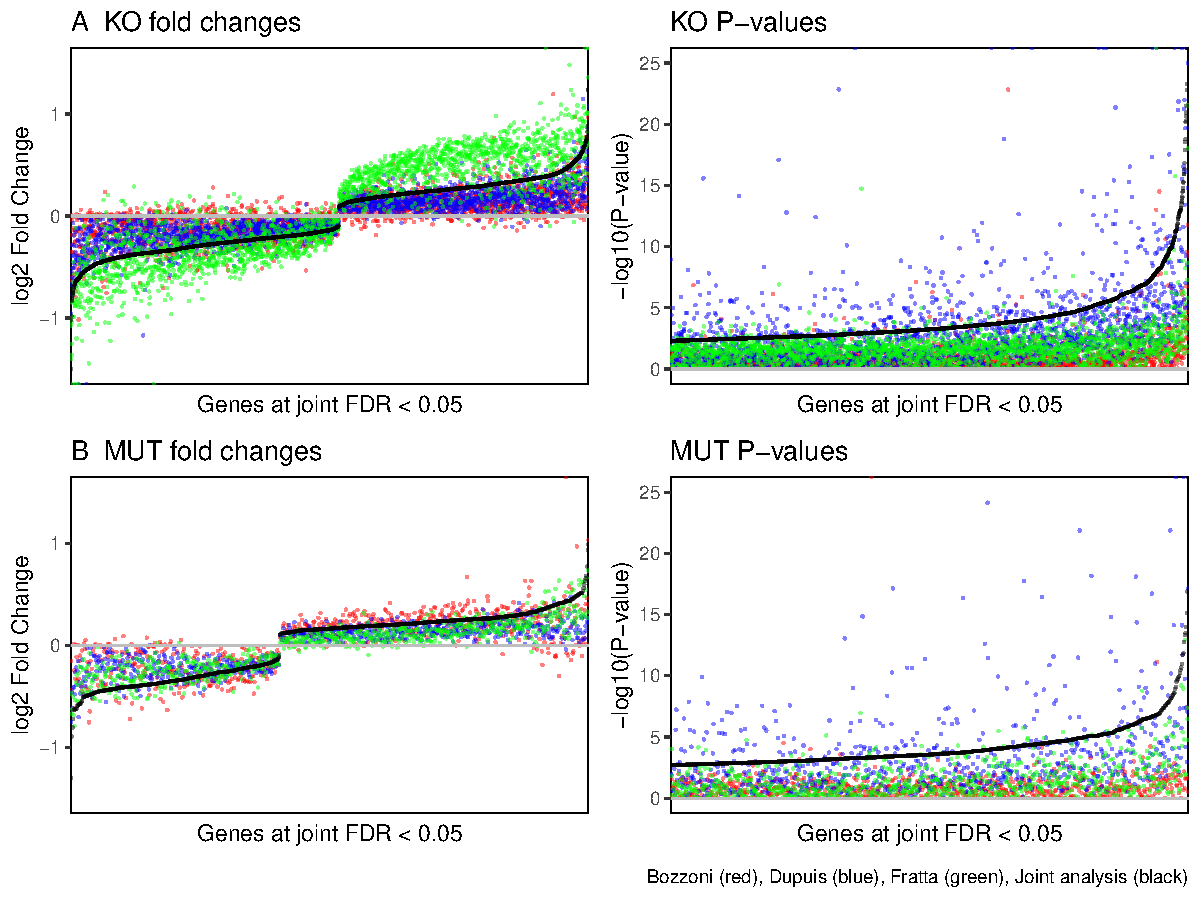
\includegraphics[width=\textwidth]{Figures/06_fus_meta/fitted_vs_individual_p_lfc.pdf}
	\caption{\textbf{Joint differential expression increases power and adjusts effect sizes}}
	A: Plotting the log2 fold changes (left) and P-values(right) for the 2136 KO genes and 754 MUT genes found at FDR < 0.05 in the two joint analyses. Values found in the individual analyses, Bozzoni (red), Dupuis(blue) and Fratta (green) are compared to the value produced by the joint analysis (black).
	B: As before but for the MUT analyses.
	\label{fig:value_comparison}
\end{figure}

For each gene the resulting joint log2 fold change and p-value is an estimated combination of the three datasets.
I compared the values found by the individual analyses with the joint models \ref{fig:value_comparison}.
For the KO models, the Fratta KO dataset has inflated log2 fold change values compared to Bozzoni and Dupuis and it is clear that the fitted log2 fold change is a compromise between the estimated fold changes of all three datasets. When inspecting the distribution of P-values, the Dupuis KO dataset has a large excess of low P-values



% Explain strict and relaxed overlap

\begin{figure}[h!]
	\centering
	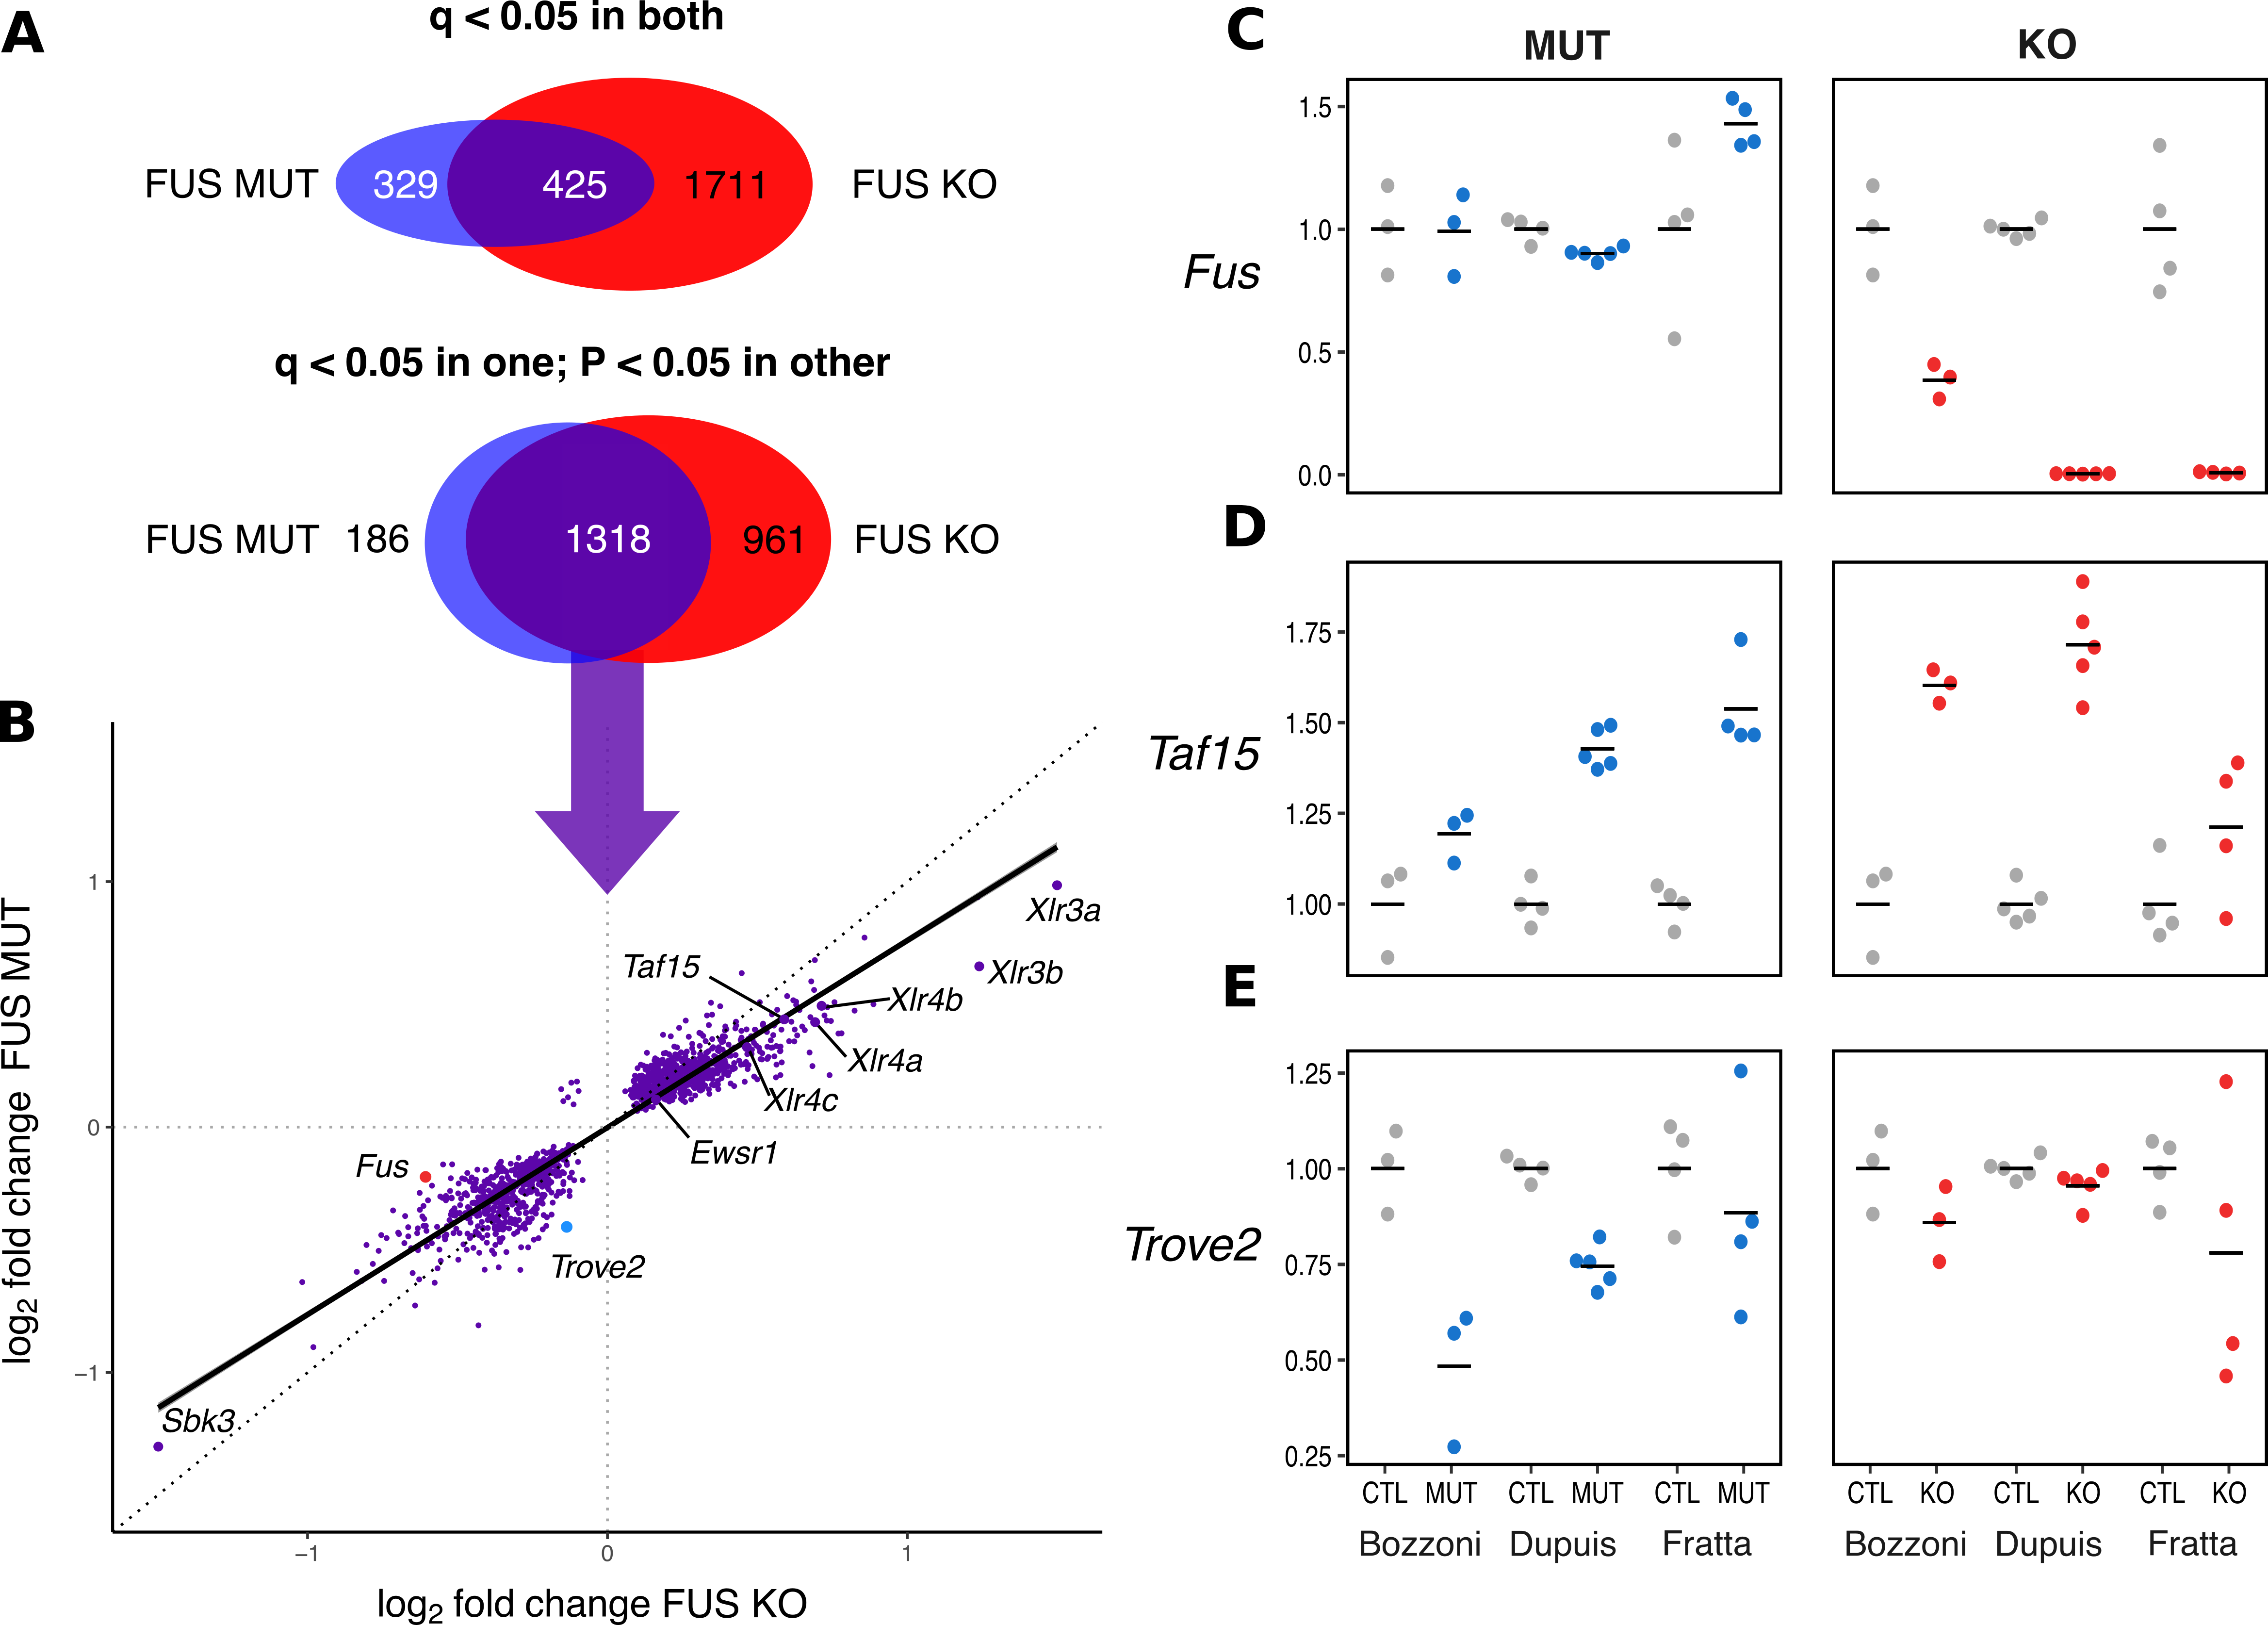
\includegraphics[width=\textwidth]{Figures/06_fus_meta/expression_multi.png}
	\caption{\textbf{Overlapping the joint differential expression models shows that FUS mutations affect gene expression in generally the same direction}}
	A: Venn diagrams show the overlap between the FUS KO and FUS MUT joint differential expression models with a strict FDR cut-off (upper) and a more relaxed P-value cut-off. 
	B: Plotting the fitted $log_2$ fold-change values for each of the 1318 overlapping genes in KO and MUT shows a bias towards weaker changes in MUT compared to KO.
	C, D,E: Normalised read counts in each dataset for \textit{Fus}, \textit{Taf15} and \textit{Trove2}. Samples are plotted relative to the mean expression in controls (CTL).
	\label{fig:fus_expression_multipanel}
\end{figure}

The two joint models provide a set of genes where we can be confident of a shared signal between all three datasets.  
I wanted to look for evidence of a shared gene expression signal between the KO model and the MUT model.
Taking a conservative threshold for overlap, where a gene must be significant at FDR < 0.05 in both models creates a moderate but convincing overlap of 425 shared genes between KO and MUT ( Figure \ref{fig:fus_expression_multipanel} A). 
If we relax our overlap criteria to FDR < 0.05 in one model and an uncorrected P < 0.05 in the other then we can see a substantial overlap where the majority of genes are now shared between KO and MUT. 
This relaxed overlap reduces the number of genes I classify as mutation-specific to 186, and knockout specific to 961.

Comparing the log$_2$ fold changes of the 1318 overlapping genes between FUS KO and FUS MUT shows that only 7 genes are altered in opposing directions (0.5\%).
The overwhelming majority of overlapping genes are altered in the same direction between FUS KO and FUS MUT.
Fitting a linear model between the two dataset's fold changes demonstates that in general the effect of FUS MUT on gene expression is 76\% that of FUS KO:

\begin{align*}
log_2FC_{mut} \sim \alpha + \beta log_2FC_{KO} \text{ } \alpha = -0.002, \beta = 0.76; P < 1e-16; \text{F-test} 
\end{align*}

This suggests that while FUS KO and FUS MUT affect the same genes in the same directions, the strength of change is greater in FUS KO than FUS MUT. This is to be expected if the changes are resulting from depletion of FUS in the nucleus. This relationship is not an artefact of the relaxed overlap criteria as fitting the model on just the 425 strictly overlapping genes results in $\beta = 0.8; P < 1e-16$.
Nuclear depletion will be stronger in the knockout than in the NLS mutations as mutant FUS is still transported to nucleus albeit at a much reduced level.

Visualising single genes in all the datasets demonstrates the power of the joint models.
It also clearly shows the increased within-condition variance for the Fratta dataset.
\textit{Fus} itself is unchanged in FUS MUT but strongly downregulated in FUS KO (Figure \ref{fig:fus_expression_multipanel}C), leading to its classification as KO specific.
The Bozzoni KO is indeed weak, with a reduction of \textit{Fus} RNA to only 40\% of wildtype, compared to near 100\% knockout in the other two datasets.
The other members of the FET family of RNA-binding proteins,  \textit{Taf15} and \textit{Ewsr1} have been shown to be bound by FUS \cite{Scekic-zahirovic2016} % other citations too.
\textit{Taf15} is strongly upregulated in both MUT and KO (Figure \ref{fig:fus_expression_multipanel}D), as is \textit{Ewsr1}.
The \textit{Trove2} gene encoding the 60 kDa SS-A/Ro ribonucleoprotein,  is downregulated in MUT only and unchanged in KO (Figure \ref{fig:fus_expression_multipanel}E), making it MUT specific.

The strongest changing genes have not been previously reported in the literature.
\textit{Sbk3}, SH3 Domain Binding Kinase Family Member 3, has the strongest negative change in both conditions. 
The X-linked lymphocyte receptor genes, \textit{Xlr3a, Xlr3b, Xlr4a} and \textit{Xlr4b} are all strongly upregulated in both conditions but more so in KO than MUT.
These genes form a cluster of paralogous genes on the X chromosome and are paternally imprinted \cite{Raefski2005}. 
As embryonic mice are not typically sexed, I was concerned that these changes were drive by an imbalance of sexes between conditions.
I was able to sex the samples \textit{in silico} using the read counts aligning to chrY-specific genes (see Appendices). 
Although there is an imbalance between sexes it is clearly not driving the large upregulation of \textit{Xlr} genes . 
The upregulation of \textit{Xlr3a} is strongest within the all-male Bozzoni dataset (Figure \ref{fig:fus_xlr_expression}A) and can also be seen in the mixed-sex Dupuis and Fratta datasets. 

\begin{figure}[h!]
	\centering
	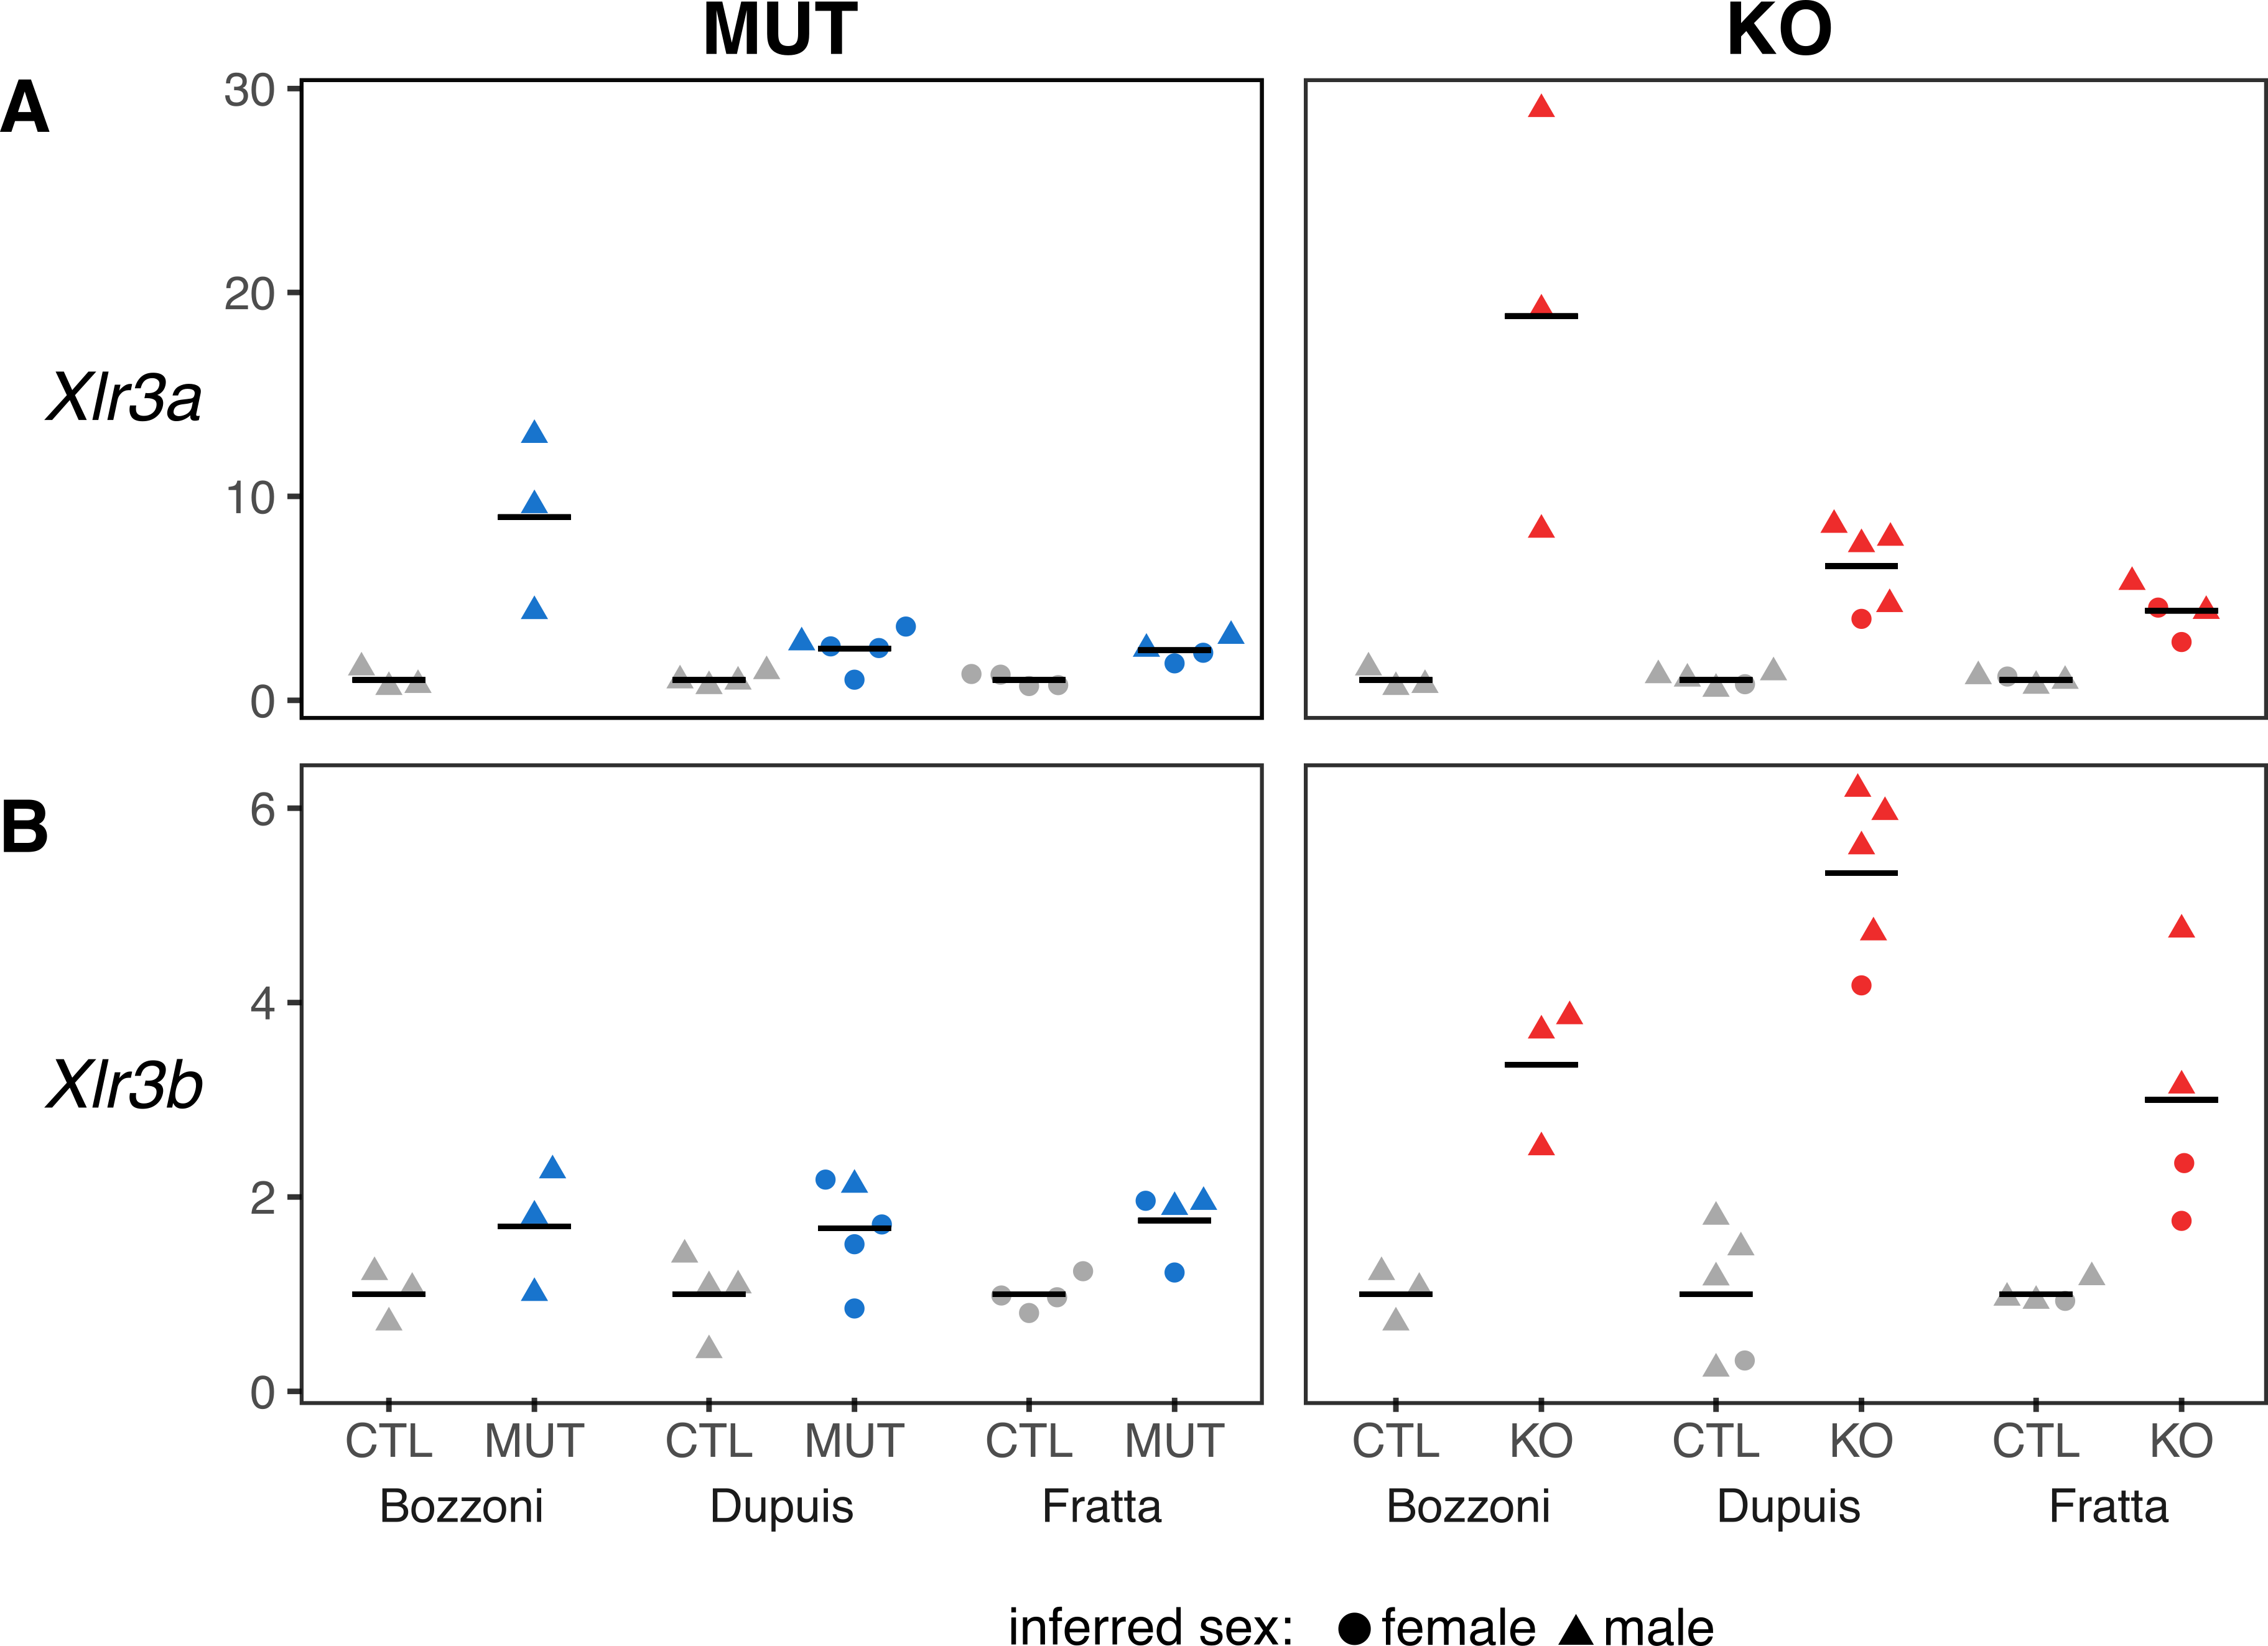
\includegraphics[width=10cm]{Figures/06_fus_meta/xlr_sex_expression.png}
	\caption{\textbf{Xlr genes are strongly upregulated in both FUS KO and FUS MUT} }	
    Normalised read counts in each dataset, plotted relative to the mean of each dataset and condition-specific control group for Xlr3a (A) and Xlr3b (B). 
	\label{fig:fus_xlr_expression}
\end{figure}


%Comparing the log2 fold changes (LFC) between KO and MUT with linear regression demonstrates that the overlapping genes are changed on average 76\% in MUT of the strength in KO. ( lfc_MUT = 0.76 . lfc_KO - 0.0017; P < 1e-16; F-test).

% opposing 7 genes
%Only 7 genes are changed in the opposite direction (0.5%). 3/7 have FUS iCLIP peaks overlapping
%Prickle2 is a synaptic gene, large number of iCLIP peaks in first 250kb intron - long gene!
%Dcaf7 has a 7 read iCLIP peak in the first intron (short intron)
%Cds2 has 2 peaks (7 and 1) in the 3'UTR


\subsection{Synaptic and RNA-binding genes are a common gene expression response to FUS nuclear depletion}

\begin{figure}[h!]
	\centering
	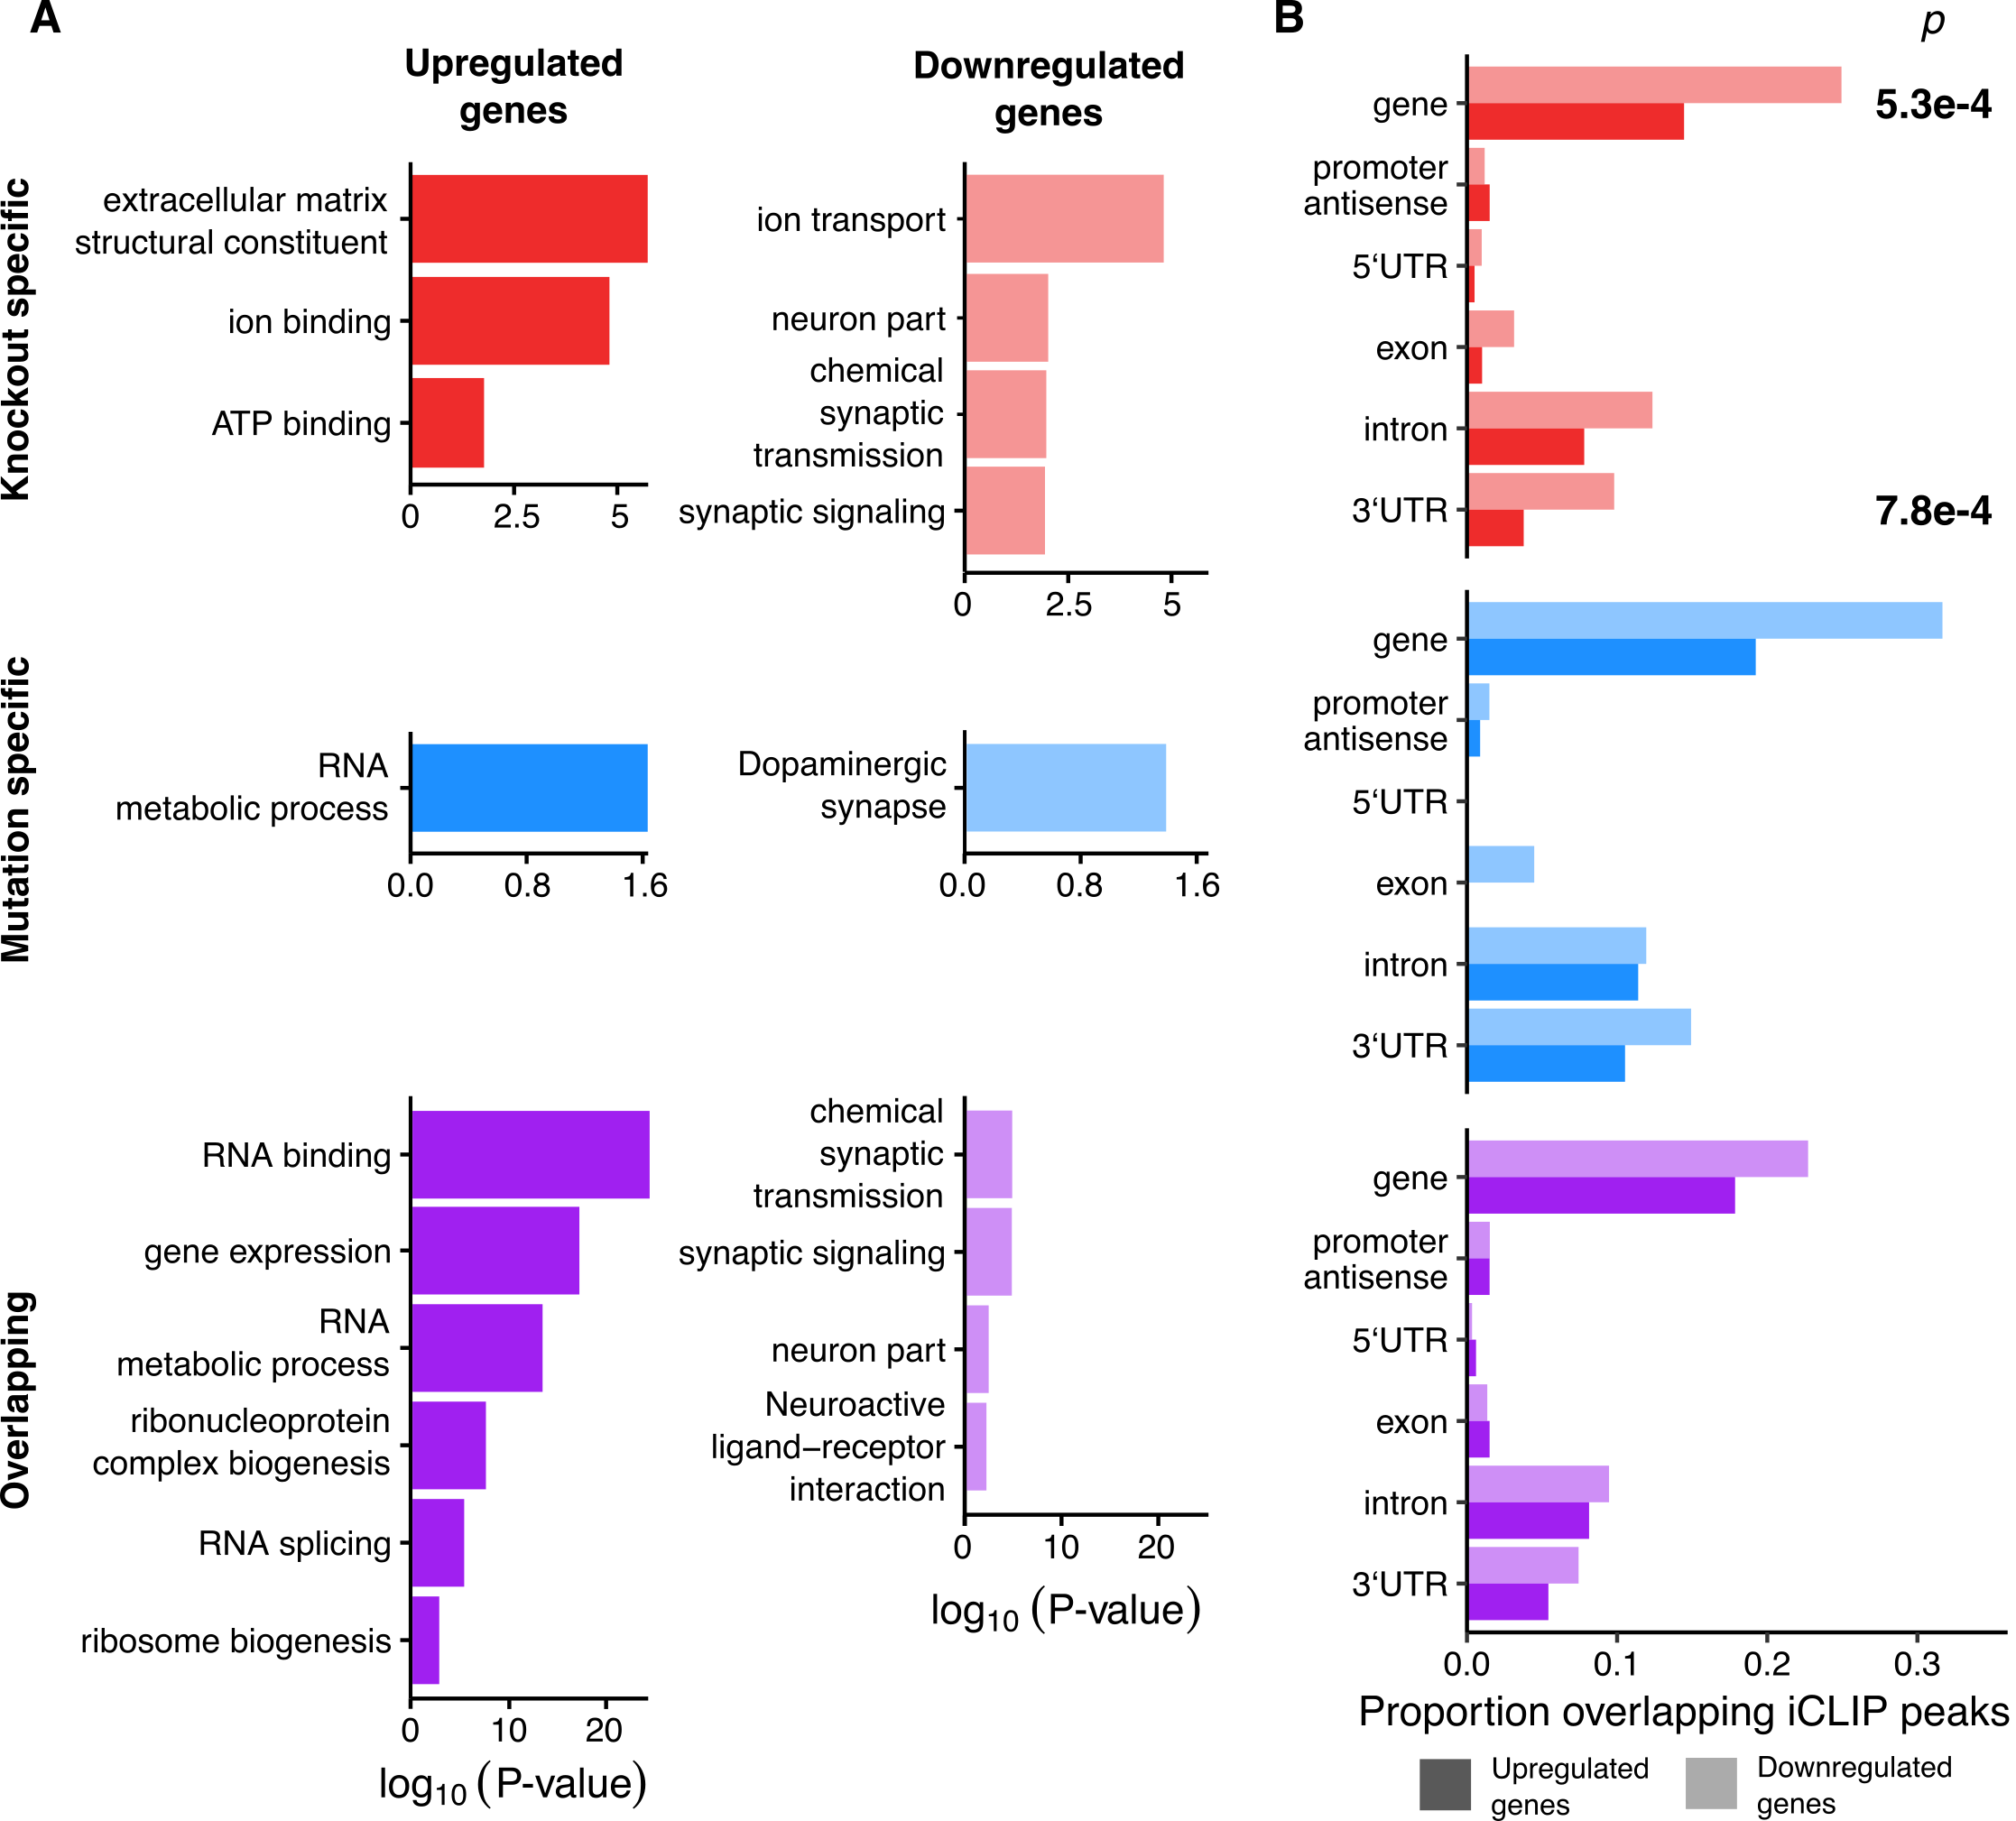
\includegraphics[width=12cm]{Figures/06_fus_meta/expression_curated_go_terms.png}
	\caption{\textbf{Overlapping genes are enriched in neuronal and RNA terms} }	
	Enriched Gene Ontology terms in the three groups of genes, split by direction.
	\label{fig:fus_expression_go}
\end{figure}


Gene ontology (GO) terms enriched in the overlapping genes were strongly direction specific, with terms involving RNA binding, splicing and metabolism enriched in upregulated genes whereas synaptic and neuronal terms were enriched in downregulated genes.

Knockout- and mutation- specific genes were less clearly enriched in specific functions. Knockout specific genes were involved in extracellular membrane functions, ion channels and amino acid transport whereas the 186 mutant specific genes showed an enrichment in Dopaminergic synapses and metabolism.

% TABLE OF GENE EXPRESSION NUMBERS
\begingroup
\renewcommand{\arraystretch}{1.5}
\begin{table}[h!]
	%\begin{centerline}
		\begin{tabular}{|r|ccc|ccc|}
			\hline
			& Bozzoni & Dupuis & Fratta & Bozzoni & Dupuis & Fratta\\[-0.3cm]
			& MUT & MUT & MUT & KO & KO & KO\\
			\hline
			Individual hits                & 19 & 1552 & 88 & 100 & 2916 & 151 \\
			Overlapping joint model & 5 & 368 & 57 & 51 & 1007 & 114 \\
			Unique to dataset          & 14 & 1184 & 31 & 49 & 1909 & 37 \\
			\hline
			\textbf{Joint model}       & \multicolumn{3}{c|}{754} & \multicolumn{3}{c|}{2136} \\
			\hline
			Overlap (strict)              & \multicolumn{2}{c}{329} & \multicolumn{2}{|c|}{\textbf{425}} & \multicolumn{2}{c|}{1711} \\
			Overlap (relaxed)           & \multicolumn{2}{c}{186} & \multicolumn{2}{|c|}{\textbf{1318} } & \multicolumn{2}{c|}{961} \\
			\hline
		\end{tabular}
	%\end{centerline}
	\caption{Results from separate and joint differential expression analysis}
	\label{tab:expression_results}
\end{table}
\endgroup


\subsection{ Overlapping genes are bound by FUS in introns and 3'UTRs}

DO ANALYSIS



\subsection{FUS modulates the inclusion of a set of highly conserved RNA-binding protein introns}

\begingroup
\renewcommand{\arraystretch}{1.5} 
\begin{table}[h!]
	%\begin{centerline}
		\begin{tabular}{|r|ccc|ccc|}
			\hline
			%\centering
			& Bozzoni & Dupuis & Fratta & Bozzoni & Dupuis & Fratta\\[-0.3cm]
			& MUT & MUT & MUT & KO & KO & KO\\
			\hline
			Individual hits                & 31 & 1 & 56 & 211 & 46 & 230 \\
			Overlapping joint model & 7 & 1 & 30 & 143 & 38 & 169 \\
			Unique to dataset          & 24 & 0 & 26 & 68 & 8 & 61 \\
			\hline
			\textbf{Joint model}       & \multicolumn{3}{c|}{93} & \multicolumn{3}{c|}{890} \\
			\hline
			Overlap (strict)              & \multicolumn{2}{c|}{33} & \multicolumn{2}{c|}{\textbf{60}} & \multicolumn{2}{c|}{830} \\
			Overlap (relaxed)           & \multicolumn{2}{c|}{16} & \multicolumn{2}{c|}{\textbf{405} } & \multicolumn{2}{c|}{501} \\
			\hline
		\end{tabular}
	%\end{centerline}
	\caption{Results from separate and joint splicing analysis}
	\label{tab:splicing_results}
\end{table}
\endgroup

\subsection{FUS autoregulation is dependent on intron retention}


\clearpage
\section{Discussion}